%\documentclass{standalone}
%\usepackage{tikz}
%\usetikzlibrary{patterns,plotmarks}
%\begin{document}
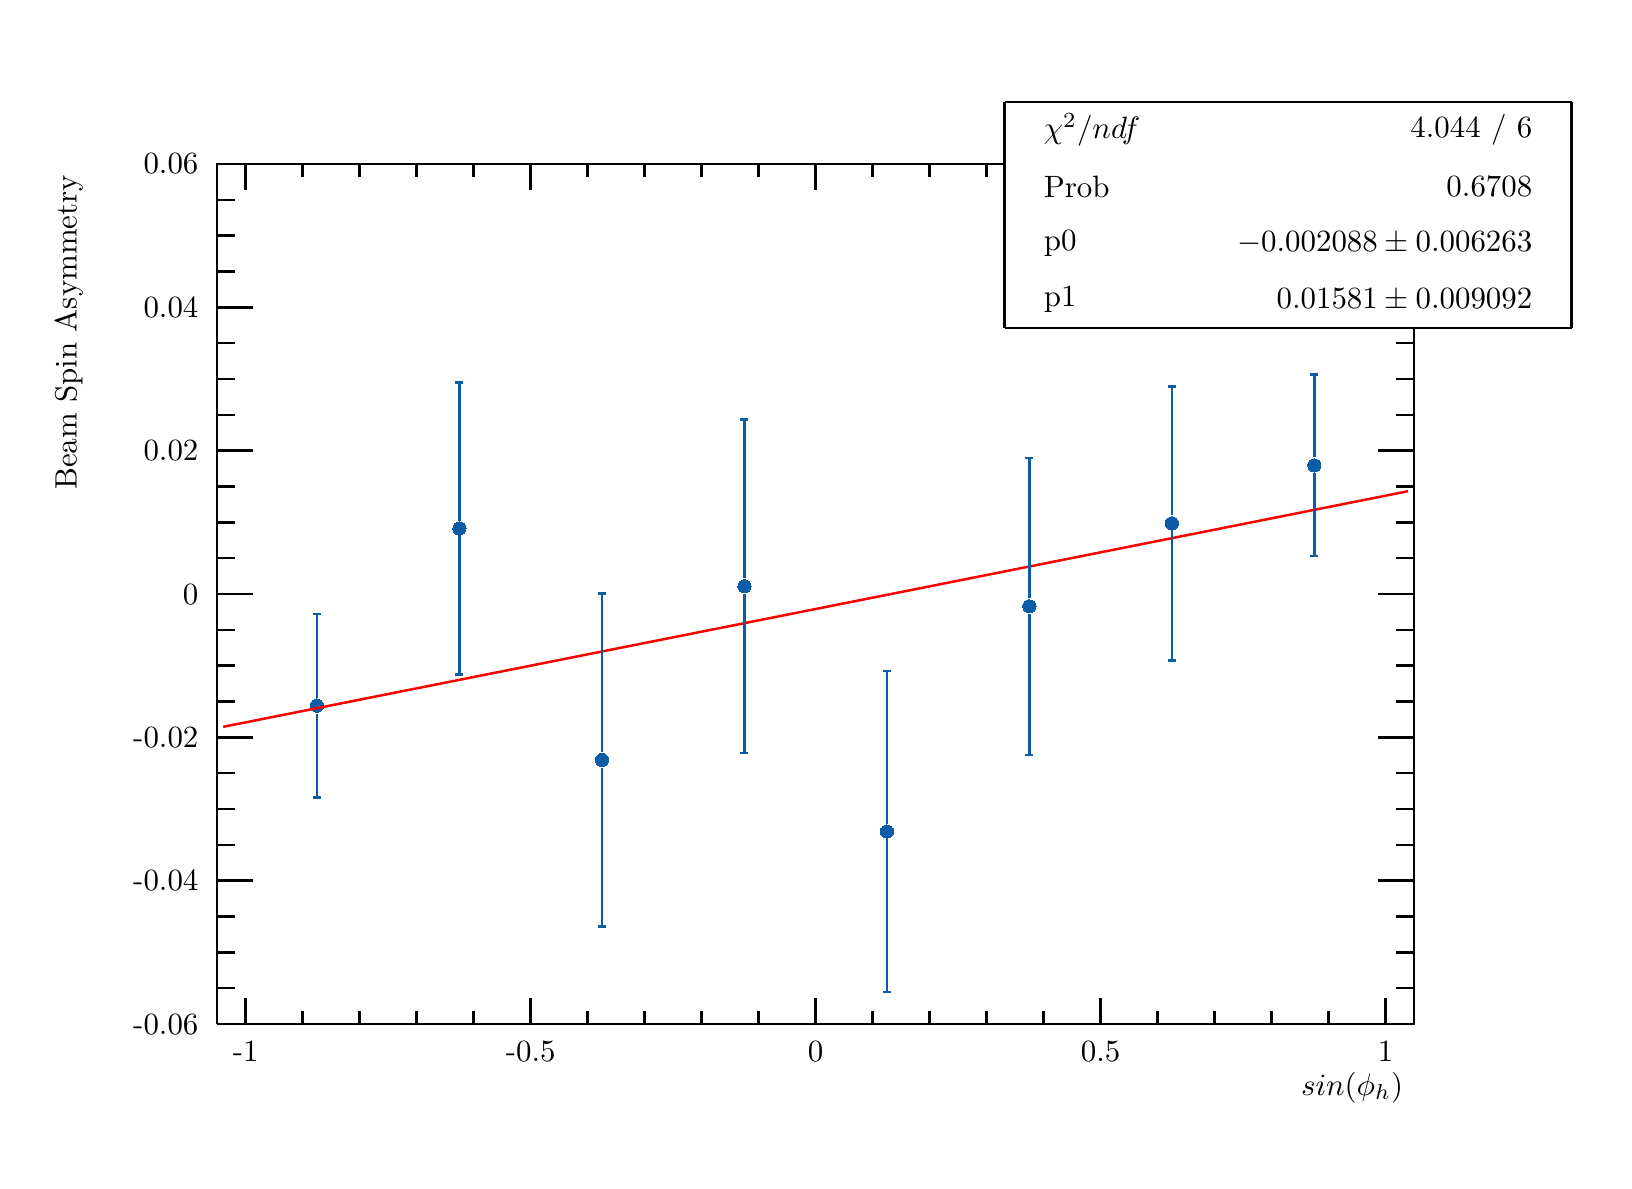
\begin{tikzpicture}
\def\CheckTikzLibraryLoaded#1{ \ifcsname tikz@library@#1@loaded\endcsname \else \PackageWarning{tikz}{usetikzlibrary{#1} is missing in the preamble.} \fi }
\CheckTikzLibraryLoaded{patterns}
\CheckTikzLibraryLoaded{plotmarks}
\pgfdeclareplotmark{cross} {
\pgfpathmoveto{\pgfpoint{-0.3\pgfplotmarksize}{\pgfplotmarksize}}
\pgfpathlineto{\pgfpoint{+0.3\pgfplotmarksize}{\pgfplotmarksize}}
\pgfpathlineto{\pgfpoint{+0.3\pgfplotmarksize}{0.3\pgfplotmarksize}}
\pgfpathlineto{\pgfpoint{+1\pgfplotmarksize}{0.3\pgfplotmarksize}}
\pgfpathlineto{\pgfpoint{+1\pgfplotmarksize}{-0.3\pgfplotmarksize}}
\pgfpathlineto{\pgfpoint{+0.3\pgfplotmarksize}{-0.3\pgfplotmarksize}}
\pgfpathlineto{\pgfpoint{+0.3\pgfplotmarksize}{-1.\pgfplotmarksize}}
\pgfpathlineto{\pgfpoint{-0.3\pgfplotmarksize}{-1.\pgfplotmarksize}}
\pgfpathlineto{\pgfpoint{-0.3\pgfplotmarksize}{-0.3\pgfplotmarksize}}
\pgfpathlineto{\pgfpoint{-1.\pgfplotmarksize}{-0.3\pgfplotmarksize}}
\pgfpathlineto{\pgfpoint{-1.\pgfplotmarksize}{0.3\pgfplotmarksize}}
\pgfpathlineto{\pgfpoint{-0.3\pgfplotmarksize}{0.3\pgfplotmarksize}}
\pgfpathclose
\pgfusepathqstroke
}
\pgfdeclareplotmark{cross*} {
\pgfpathmoveto{\pgfpoint{-0.3\pgfplotmarksize}{\pgfplotmarksize}}
\pgfpathlineto{\pgfpoint{+0.3\pgfplotmarksize}{\pgfplotmarksize}}
\pgfpathlineto{\pgfpoint{+0.3\pgfplotmarksize}{0.3\pgfplotmarksize}}
\pgfpathlineto{\pgfpoint{+1\pgfplotmarksize}{0.3\pgfplotmarksize}}
\pgfpathlineto{\pgfpoint{+1\pgfplotmarksize}{-0.3\pgfplotmarksize}}
\pgfpathlineto{\pgfpoint{+0.3\pgfplotmarksize}{-0.3\pgfplotmarksize}}
\pgfpathlineto{\pgfpoint{+0.3\pgfplotmarksize}{-1.\pgfplotmarksize}}
\pgfpathlineto{\pgfpoint{-0.3\pgfplotmarksize}{-1.\pgfplotmarksize}}
\pgfpathlineto{\pgfpoint{-0.3\pgfplotmarksize}{-0.3\pgfplotmarksize}}
\pgfpathlineto{\pgfpoint{-1.\pgfplotmarksize}{-0.3\pgfplotmarksize}}
\pgfpathlineto{\pgfpoint{-1.\pgfplotmarksize}{0.3\pgfplotmarksize}}
\pgfpathlineto{\pgfpoint{-0.3\pgfplotmarksize}{0.3\pgfplotmarksize}}
\pgfpathclose
\pgfusepathqfillstroke
}
\pgfdeclareplotmark{newstar} {
\pgfpathmoveto{\pgfqpoint{0pt}{\pgfplotmarksize}}
\pgfpathlineto{\pgfqpointpolar{44}{0.5\pgfplotmarksize}}
\pgfpathlineto{\pgfqpointpolar{18}{\pgfplotmarksize}}
\pgfpathlineto{\pgfqpointpolar{-20}{0.5\pgfplotmarksize}}
\pgfpathlineto{\pgfqpointpolar{-54}{\pgfplotmarksize}}
\pgfpathlineto{\pgfqpointpolar{-90}{0.5\pgfplotmarksize}}
\pgfpathlineto{\pgfqpointpolar{234}{\pgfplotmarksize}}
\pgfpathlineto{\pgfqpointpolar{198}{0.5\pgfplotmarksize}}
\pgfpathlineto{\pgfqpointpolar{162}{\pgfplotmarksize}}
\pgfpathlineto{\pgfqpointpolar{134}{0.5\pgfplotmarksize}}
\pgfpathclose
\pgfusepathqstroke
}
\pgfdeclareplotmark{newstar*} {
\pgfpathmoveto{\pgfqpoint{0pt}{\pgfplotmarksize}}
\pgfpathlineto{\pgfqpointpolar{44}{0.5\pgfplotmarksize}}
\pgfpathlineto{\pgfqpointpolar{18}{\pgfplotmarksize}}
\pgfpathlineto{\pgfqpointpolar{-20}{0.5\pgfplotmarksize}}
\pgfpathlineto{\pgfqpointpolar{-54}{\pgfplotmarksize}}
\pgfpathlineto{\pgfqpointpolar{-90}{0.5\pgfplotmarksize}}
\pgfpathlineto{\pgfqpointpolar{234}{\pgfplotmarksize}}
\pgfpathlineto{\pgfqpointpolar{198}{0.5\pgfplotmarksize}}
\pgfpathlineto{\pgfqpointpolar{162}{\pgfplotmarksize}}
\pgfpathlineto{\pgfqpointpolar{134}{0.5\pgfplotmarksize}}
\pgfpathclose
\pgfusepathqfillstroke
}
\definecolor{c}{rgb}{1,1,1};
\draw [color=c, fill=c] (0,0) rectangle (20,14.3719);
\draw [color=c, fill=c] (2.4,1.72462) rectangle (17.6,12.6472);
\definecolor{c}{rgb}{0,0,0};
\draw [c,line width=0.9] (2.4,1.72462) -- (2.4,12.6472) -- (17.6,12.6472) -- (17.6,1.72462) -- (2.4,1.72462);
\definecolor{c}{rgb}{1,1,1};
\draw [color=c, fill=c] (2.4,1.72462) rectangle (17.6,12.6472);
\definecolor{c}{rgb}{0,0,0};
\draw [c,line width=0.9] (2.4,1.72462) -- (2.4,12.6472) -- (17.6,12.6472) -- (17.6,1.72462) -- (2.4,1.72462);
\draw [c,line width=0.9] (2.4,1.72462) -- (17.6,1.72462);
\draw [c,line width=0.9] (2.7619,2.0523) -- (2.7619,1.72462);
\draw [c,line width=0.9] (3.48571,1.88846) -- (3.48571,1.72462);
\draw [c,line width=0.9] (4.20952,1.88846) -- (4.20952,1.72462);
\draw [c,line width=0.9] (4.93333,1.88846) -- (4.93333,1.72462);
\draw [c,line width=0.9] (5.65714,1.88846) -- (5.65714,1.72462);
\draw [c,line width=0.9] (6.38095,2.0523) -- (6.38095,1.72462);
\draw [c,line width=0.9] (7.10476,1.88846) -- (7.10476,1.72462);
\draw [c,line width=0.9] (7.82857,1.88846) -- (7.82857,1.72462);
\draw [c,line width=0.9] (8.55238,1.88846) -- (8.55238,1.72462);
\draw [c,line width=0.9] (9.27619,1.88846) -- (9.27619,1.72462);
\draw [c,line width=0.9] (10,2.0523) -- (10,1.72462);
\draw [c,line width=0.9] (10.7238,1.88846) -- (10.7238,1.72462);
\draw [c,line width=0.9] (11.4476,1.88846) -- (11.4476,1.72462);
\draw [c,line width=0.9] (12.1714,1.88846) -- (12.1714,1.72462);
\draw [c,line width=0.9] (12.8952,1.88846) -- (12.8952,1.72462);
\draw [c,line width=0.9] (13.619,2.0523) -- (13.619,1.72462);
\draw [c,line width=0.9] (14.3429,1.88846) -- (14.3429,1.72462);
\draw [c,line width=0.9] (15.0667,1.88846) -- (15.0667,1.72462);
\draw [c,line width=0.9] (15.7905,1.88846) -- (15.7905,1.72462);
\draw [c,line width=0.9] (16.5143,1.88846) -- (16.5143,1.72462);
\draw [c,line width=0.9] (17.2381,2.0523) -- (17.2381,1.72462);
\draw [c,line width=0.9] (2.7619,2.0523) -- (2.7619,1.72462);
\draw [c,line width=0.9] (17.2381,2.0523) -- (17.2381,1.72462);
\draw [anchor=base] (2.7619,1.25035) node[scale=1.11607, color=c, rotate=0]{-1};
\draw [anchor=base] (6.38095,1.25035) node[scale=1.11607, color=c, rotate=0]{-0.5};
\draw [anchor=base] (10,1.25035) node[scale=1.11607, color=c, rotate=0]{0};
\draw [anchor=base] (13.619,1.25035) node[scale=1.11607, color=c, rotate=0]{0.5};
\draw [anchor=base] (17.2381,1.25035) node[scale=1.11607, color=c, rotate=0]{1};
\draw [anchor= east] (17.6,0.919799) node[scale=1.11607, color=c, rotate=0]{$sin(\phi_{h})$};
\draw [c,line width=0.9] (2.4,12.6472) -- (17.6,12.6472);
\draw [c,line width=0.9] (2.7619,12.3196) -- (2.7619,12.6472);
\draw [c,line width=0.9] (3.48571,12.4834) -- (3.48571,12.6472);
\draw [c,line width=0.9] (4.20952,12.4834) -- (4.20952,12.6472);
\draw [c,line width=0.9] (4.93333,12.4834) -- (4.93333,12.6472);
\draw [c,line width=0.9] (5.65714,12.4834) -- (5.65714,12.6472);
\draw [c,line width=0.9] (6.38095,12.3196) -- (6.38095,12.6472);
\draw [c,line width=0.9] (7.10476,12.4834) -- (7.10476,12.6472);
\draw [c,line width=0.9] (7.82857,12.4834) -- (7.82857,12.6472);
\draw [c,line width=0.9] (8.55238,12.4834) -- (8.55238,12.6472);
\draw [c,line width=0.9] (9.27619,12.4834) -- (9.27619,12.6472);
\draw [c,line width=0.9] (10,12.3196) -- (10,12.6472);
\draw [c,line width=0.9] (10.7238,12.4834) -- (10.7238,12.6472);
\draw [c,line width=0.9] (11.4476,12.4834) -- (11.4476,12.6472);
\draw [c,line width=0.9] (12.1714,12.4834) -- (12.1714,12.6472);
\draw [c,line width=0.9] (12.8952,12.4834) -- (12.8952,12.6472);
\draw [c,line width=0.9] (13.619,12.3196) -- (13.619,12.6472);
\draw [c,line width=0.9] (14.3429,12.4834) -- (14.3429,12.6472);
\draw [c,line width=0.9] (15.0667,12.4834) -- (15.0667,12.6472);
\draw [c,line width=0.9] (15.7905,12.4834) -- (15.7905,12.6472);
\draw [c,line width=0.9] (16.5143,12.4834) -- (16.5143,12.6472);
\draw [c,line width=0.9] (17.2381,12.3196) -- (17.2381,12.6472);
\draw [c,line width=0.9] (2.7619,12.3196) -- (2.7619,12.6472);
\draw [c,line width=0.9] (17.2381,12.3196) -- (17.2381,12.6472);
\draw [c,line width=0.9] (2.4,1.72462) -- (2.4,12.6472);
\draw [c,line width=0.9] (2.856,1.72462) -- (2.4,1.72462);
\draw [c,line width=0.9] (2.628,2.17973) -- (2.4,2.17973);
\draw [c,line width=0.9] (2.628,2.63484) -- (2.4,2.63484);
\draw [c,line width=0.9] (2.628,3.08995) -- (2.4,3.08995);
\draw [c,line width=0.9] (2.856,3.54506) -- (2.4,3.54506);
\draw [c,line width=0.9] (2.628,4.00017) -- (2.4,4.00017);
\draw [c,line width=0.9] (2.628,4.45528) -- (2.4,4.45528);
\draw [c,line width=0.9] (2.628,4.91039) -- (2.4,4.91039);
\draw [c,line width=0.9] (2.856,5.36549) -- (2.4,5.36549);
\draw [c,line width=0.9] (2.628,5.8206) -- (2.4,5.8206);
\draw [c,line width=0.9] (2.628,6.27571) -- (2.4,6.27571);
\draw [c,line width=0.9] (2.628,6.73082) -- (2.4,6.73082);
\draw [c,line width=0.9] (2.856,7.18593) -- (2.4,7.18593);
\draw [c,line width=0.9] (2.628,7.64104) -- (2.4,7.64104);
\draw [c,line width=0.9] (2.628,8.09615) -- (2.4,8.09615);
\draw [c,line width=0.9] (2.628,8.55126) -- (2.4,8.55126);
\draw [c,line width=0.9] (2.856,9.00637) -- (2.4,9.00637);
\draw [c,line width=0.9] (2.628,9.46147) -- (2.4,9.46147);
\draw [c,line width=0.9] (2.628,9.91658) -- (2.4,9.91658);
\draw [c,line width=0.9] (2.628,10.3717) -- (2.4,10.3717);
\draw [c,line width=0.9] (2.856,10.8268) -- (2.4,10.8268);
\draw [c,line width=0.9] (2.628,11.2819) -- (2.4,11.2819);
\draw [c,line width=0.9] (2.628,11.737) -- (2.4,11.737);
\draw [c,line width=0.9] (2.628,12.1921) -- (2.4,12.1921);
\draw [c,line width=0.9] (2.856,12.6472) -- (2.4,12.6472);
\draw [anchor= east] (2.3,1.72462) node[scale=1.11607, color=c, rotate=0]{-0.06};
\draw [anchor= east] (2.3,3.54506) node[scale=1.11607, color=c, rotate=0]{-0.04};
\draw [anchor= east] (2.3,5.36549) node[scale=1.11607, color=c, rotate=0]{-0.02};
\draw [anchor= east] (2.3,7.18593) node[scale=1.11607, color=c, rotate=0]{0};
\draw [anchor= east] (2.3,9.00637) node[scale=1.11607, color=c, rotate=0]{0.02};
\draw [anchor= east] (2.3,10.8268) node[scale=1.11607, color=c, rotate=0]{0.04};
\draw [anchor= east] (2.3,12.6472) node[scale=1.11607, color=c, rotate=0]{0.06};
\draw [anchor= east] (0.519095,12.6472) node[scale=1.11607, color=c, rotate=90]{Beam Spin Asymmetry};
\draw [c,line width=0.9] (17.6,1.72462) -- (17.6,12.6472);
\draw [c,line width=0.9] (17.144,1.72462) -- (17.6,1.72462);
\draw [c,line width=0.9] (17.372,2.17973) -- (17.6,2.17973);
\draw [c,line width=0.9] (17.372,2.63484) -- (17.6,2.63484);
\draw [c,line width=0.9] (17.372,3.08995) -- (17.6,3.08995);
\draw [c,line width=0.9] (17.144,3.54506) -- (17.6,3.54506);
\draw [c,line width=0.9] (17.372,4.00017) -- (17.6,4.00017);
\draw [c,line width=0.9] (17.372,4.45528) -- (17.6,4.45528);
\draw [c,line width=0.9] (17.372,4.91039) -- (17.6,4.91039);
\draw [c,line width=0.9] (17.144,5.36549) -- (17.6,5.36549);
\draw [c,line width=0.9] (17.372,5.8206) -- (17.6,5.8206);
\draw [c,line width=0.9] (17.372,6.27571) -- (17.6,6.27571);
\draw [c,line width=0.9] (17.372,6.73082) -- (17.6,6.73082);
\draw [c,line width=0.9] (17.144,7.18593) -- (17.6,7.18593);
\draw [c,line width=0.9] (17.372,7.64104) -- (17.6,7.64104);
\draw [c,line width=0.9] (17.372,8.09615) -- (17.6,8.09615);
\draw [c,line width=0.9] (17.372,8.55126) -- (17.6,8.55126);
\draw [c,line width=0.9] (17.144,9.00637) -- (17.6,9.00637);
\draw [c,line width=0.9] (17.372,9.46147) -- (17.6,9.46147);
\draw [c,line width=0.9] (17.372,9.91658) -- (17.6,9.91658);
\draw [c,line width=0.9] (17.372,10.3717) -- (17.6,10.3717);
\draw [c,line width=0.9] (17.144,10.8268) -- (17.6,10.8268);
\draw [c,line width=0.9] (17.372,11.2819) -- (17.6,11.2819);
\draw [c,line width=0.9] (17.372,11.737) -- (17.6,11.737);
\draw [c,line width=0.9] (17.372,12.1921) -- (17.6,12.1921);
\draw [c,line width=0.9] (17.144,12.6472) -- (17.6,12.6472);
\definecolor{c}{rgb}{0.0470588,0.364706,0.647059};
\foreach \P in {(3.66667,5.76907), (5.47619,8.01822), (7.28571,5.07826), (9.09524,7.28444), (10.9048,4.17015), (12.7143,7.02967), (14.5238,8.08319), (16.3333,8.81965)}{\draw[mark options={color=c,fill=c},mark size=2.402402pt, line width=0.000000pt,
 mark=*] plot coordinates {\P};}
\definecolor{c}{rgb}{1,0,0};
\draw [c,line width=0.9] (2.476,5.49975) -- (2.628,5.52997) -- (2.78,5.56019) -- (2.932,5.59042) -- (3.084,5.62064) -- (3.236,5.65087) -- (3.388,5.68109) -- (3.54,5.71132) -- (3.692,5.74154) -- (3.844,5.77177) -- (3.996,5.80199) -- (4.148,5.83222) --
 (4.3,5.86244) -- (4.452,5.89267) -- (4.604,5.92289) -- (4.756,5.95312) -- (4.908,5.98334) -- (5.06,6.01357) -- (5.212,6.04379) -- (5.364,6.07402) -- (5.516,6.10424) -- (5.668,6.13447) -- (5.82,6.16469) -- (5.972,6.19492) -- (6.124,6.22514) --
 (6.276,6.25537) -- (6.428,6.28559) -- (6.58,6.31582) -- (6.732,6.34604) -- (6.884,6.37627) -- (7.036,6.40649) -- (7.188,6.43672) -- (7.34,6.46694) -- (7.492,6.49716) -- (7.644,6.52739) -- (7.796,6.55761) -- (7.948,6.58784) -- (8.1,6.61806) --
 (8.252,6.64829) -- (8.404,6.67851) -- (8.556,6.70874) -- (8.708,6.73896) -- (8.86,6.76919) -- (9.012,6.79941) -- (9.164,6.82964) -- (9.316,6.85986) -- (9.468,6.89009) -- (9.62,6.92031) -- (9.772,6.95054) -- (9.924,6.98076);
\draw [c,line width=0.9] (9.924,6.98076) -- (10.076,7.01099) -- (10.228,7.04121) -- (10.38,7.07144) -- (10.532,7.10166) -- (10.684,7.13189) -- (10.836,7.16211) -- (10.988,7.19234) -- (11.14,7.22256) -- (11.292,7.25279) -- (11.444,7.28301) --
 (11.596,7.31324) -- (11.748,7.34346) -- (11.9,7.37368) -- (12.052,7.40391) -- (12.204,7.43413) -- (12.356,7.46436) -- (12.508,7.49458) -- (12.66,7.52481) -- (12.812,7.55503) -- (12.964,7.58526) -- (13.116,7.61548) -- (13.268,7.64571) --
 (13.42,7.67593) -- (13.572,7.70616) -- (13.724,7.73638) -- (13.876,7.76661) -- (14.028,7.79683) -- (14.18,7.82706) -- (14.332,7.85728) -- (14.484,7.88751) -- (14.636,7.91773) -- (14.788,7.94796) -- (14.94,7.97818) -- (15.092,8.00841) --
 (15.244,8.03863) -- (15.396,8.06886) -- (15.548,8.09908) -- (15.7,8.12931) -- (15.852,8.15953) -- (16.004,8.18976) -- (16.156,8.21998) -- (16.308,8.25021) -- (16.46,8.28043) -- (16.612,8.31065) -- (16.764,8.34088) -- (16.916,8.3711) --
 (17.068,8.40133) -- (17.22,8.43155) -- (17.372,8.46178);
\draw [c,line width=0.9] (17.372,8.46178) -- (17.524,8.492);
\definecolor{c}{rgb}{1,1,1};
\draw [color=c, fill=c] (12.4,10.5633) rectangle (19.6,13.4377);
\definecolor{c}{rgb}{0,0,0};
\draw [c,line width=0.9] (12.4,10.5633) -- (19.6,10.5633);
\draw [c,line width=0.9] (19.6,10.5633) -- (19.6,13.4377);
\draw [c,line width=0.9] (19.6,13.4377) -- (12.4,13.4377);
\draw [c,line width=0.9] (12.4,13.4377) -- (12.4,10.5633);
\draw [anchor= west] (12.76,13.0784) node[scale=1.11607, color=c, rotate=0]{$\chi^{2} / ndf $};
\draw [anchor= east] (19.24,13.0784) node[scale=1.11607, color=c, rotate=0]{ 4.044 / 6};
\draw [anchor= west] (12.76,12.3598) node[scale=1.11607, color=c, rotate=0]{Prob  };
\draw [anchor= east] (19.24,12.3598) node[scale=1.11607, color=c, rotate=0]{ 0.6708};
\draw [anchor= west] (12.76,11.6412) node[scale=1.11607, color=c, rotate=0]{p0       };
\draw [anchor= east] (19.24,11.6412) node[scale=1.11607, color=c, rotate=0]{$ -0.002088 \pm 0.006263$};
\draw [anchor= west] (12.76,10.9226) node[scale=1.11607, color=c, rotate=0]{p1       };
\draw [anchor= east] (19.24,10.9226) node[scale=1.11607, color=c, rotate=0]{$ 0.01581 \pm 0.009092$};
\definecolor{c}{rgb}{0.0470588,0.364706,0.647059};
\draw [c,line width=0.9] (3.66667,5.86958) -- (3.66667,6.9342);
\draw [c,line width=0.9] (3.66667,5.66857) -- (3.66667,4.60395);
\draw [c,line width=0.9] (3.61642,6.9342) -- (3.71692,6.9342);
\draw [c,line width=0.9] (3.61642,4.60395) -- (3.71692,4.60395);
\draw [c,line width=0.9] (5.47619,8.11872) -- (5.47619,9.87387);
\draw [c,line width=0.9] (5.47619,7.91771) -- (5.47619,6.16256);
\draw [c,line width=0.9] (5.42594,9.87387) -- (5.52644,9.87387);
\draw [c,line width=0.9] (5.42594,6.16256) -- (5.52644,6.16256);
\draw [c,line width=0.9] (7.28571,5.17877) -- (7.28571,7.19048);
\draw [c,line width=0.9] (7.28571,4.97776) -- (7.28571,2.96604);
\draw [c,line width=0.9] (7.23546,7.19048) -- (7.33597,7.19048);
\draw [c,line width=0.9] (7.23546,2.96604) -- (7.33597,2.96604);
\draw [c,line width=0.9] (9.09524,7.38494) -- (9.09524,9.4018);
\draw [c,line width=0.9] (9.09524,7.18394) -- (9.09524,5.16708);
\draw [c,line width=0.9] (9.04499,9.4018) -- (9.14549,9.4018);
\draw [c,line width=0.9] (9.04499,5.16708) -- (9.14549,5.16708);
\draw [c,line width=0.9] (10.9048,4.27065) -- (10.9048,6.20954);
\draw [c,line width=0.9] (10.9048,4.06965) -- (10.9048,2.13076);
\draw [c,line width=0.9] (10.8545,6.20954) -- (10.955,6.20954);
\draw [c,line width=0.9] (10.8545,2.13076) -- (10.955,2.13076);
\draw [c,line width=0.9] (12.7143,7.13017) -- (12.7143,8.91535);
\draw [c,line width=0.9] (12.7143,6.92917) -- (12.7143,5.14399);
\draw [c,line width=0.9] (12.664,8.91535) -- (12.7645,8.91535);
\draw [c,line width=0.9] (12.664,5.14399) -- (12.7645,5.14399);
\draw [c,line width=0.9] (14.5238,8.18369) -- (14.5238,9.82239);
\draw [c,line width=0.9] (14.5238,7.98268) -- (14.5238,6.34399);
\draw [c,line width=0.9] (14.4736,9.82239) -- (14.5741,9.82239);
\draw [c,line width=0.9] (14.4736,6.34399) -- (14.5741,6.34399);
\draw [c,line width=0.9] (16.3333,8.92016) -- (16.3333,9.97192);
\draw [c,line width=0.9] (16.3333,8.71915) -- (16.3333,7.66739);
\draw [c,line width=0.9] (16.2831,9.97192) -- (16.3836,9.97192);
\draw [c,line width=0.9] (16.2831,7.66739) -- (16.3836,7.66739);
\definecolor{c}{rgb}{1,1,1};
\draw [color=c, fill=c] (12.4,10.5633) rectangle (19.6,13.4377);
\definecolor{c}{rgb}{0,0,0};
\draw [c,line width=0.9] (12.4,10.5633) -- (19.6,10.5633);
\draw [c,line width=0.9] (19.6,10.5633) -- (19.6,13.4377);
\draw [c,line width=0.9] (19.6,13.4377) -- (12.4,13.4377);
\draw [c,line width=0.9] (12.4,13.4377) -- (12.4,10.5633);
\draw [anchor= west] (12.76,13.0784) node[scale=1.11607, color=c, rotate=0]{$\chi^{2} / ndf $};
\draw [anchor= east] (19.24,13.0784) node[scale=1.11607, color=c, rotate=0]{ 4.044 / 6};
\draw [anchor= west] (12.76,12.3598) node[scale=1.11607, color=c, rotate=0]{Prob  };
\draw [anchor= east] (19.24,12.3598) node[scale=1.11607, color=c, rotate=0]{ 0.6708};
\draw [anchor= west] (12.76,11.6412) node[scale=1.11607, color=c, rotate=0]{p0       };
\draw [anchor= east] (19.24,11.6412) node[scale=1.11607, color=c, rotate=0]{$ -0.002088 \pm 0.006263$};
\draw [anchor= west] (12.76,10.9226) node[scale=1.11607, color=c, rotate=0]{p1       };
\draw [anchor= east] (19.24,10.9226) node[scale=1.11607, color=c, rotate=0]{$ 0.01581 \pm 0.009092$};
\end{tikzpicture}
%\end{document}
